A Figura~\ref{fig:fluxo-pap} oferece uma leitura do funcionamento antes das telas. O caminho principal não exige salvar favorito; essa é uma ação auxiliar. O acesso por QR Code ou link direto atende à consulta dos próximos ônibus de um ponto já identificado. No mapa, clicar em um ponto durante a seleção de embarque define a origem e mantém o mapa aberto para escolher o destino; clicar durante a seleção de destino abre as alternativas de viagem. O toque prolongado em outro local segue a mesma distinção entre origem e destino. Esses comportamentos atendem a objetivos diferentes, sem obrigar a consulta de partidas antes de planejar uma viagem. Com localização conhecida, o fluxo pode começar diretamente pela seleção de destino. A chegada de novas alternativas não exige abandonar o mapa. O fluxograma sintetiza o uso e não representa todas as mensagens e transições internas.

\begin{figure}[H]
\centering\begin{tikzpicture}[>=Stealth,font=\fontsize{8}{10}\selectfont,
box/.style={draw,rounded corners,align=center,text width=3.6cm,minimum height=.8cm,fill=black!3},arr/.style={->,thick},lab/.style={font=\scriptsize,fill=white,align=center}]
\node[box] (qr) at (0,0) {QR Code ou link do ponto};
\node[box] (manual) at (4.3,0) {Selecionar embarque no mapa\\(ponto ou toque prolongado)};
\node[box] (gps) at (8.6,0) {Geolocalização disponível\\sem embarque manual ou QR};
\node[box,fill=blue!5] (times) at (0,-1.4) {Abrir próximos ônibus\\do ponto identificado};
\node[box] (stay) at (4.3,-1.4) {Definir embarque;\\permanecer no mapa};
\node[box] (auto) at (8.6,-1.4) {Usar localização como origem};
\foreach \a/\b in {qr/times,manual/stay,gps/auto}{\draw[arr] (\a)--(\b);}
\node[box,text width=5cm] (check) at (4.3,-3.2) {Ao escolher destino no mapa:\\origem disponível?};
\draw[arr] (times.south)--(0,-2.4)--node[lab,above]{se desejar planejar}(4.3,-2.4)--(check.north);
\draw[thick] (stay)--(4.3,-2.4);
\draw[thick] (auto.south)--(8.6,-2.4)--(4.3,-2.4);
\node[box,text width=2.9cm] (missing) at (-.6,-3.2) {Não: alertar e solicitar embarque};
\draw[arr] (check)--(missing);
\draw[arr] (missing.west)--(-2.5,-3.2)--(-2.5,.7)--(4.3,.7)--(manual.north);
\node[box,text width=5cm] (dest) at (4.3,-4.6) {Sim: definir destino\\ponto, toque prolongado, busca ou favorito};
\draw[arr] (check)--(dest);
\node[box,text width=5cm] (calc) at (4.3,-6) {Abrir lista de rotas;\\calcular alternativas progressivamente};
\draw[arr] (dest)--(calc);
\node[box,text width=2.5cm] (fail) at (-.6,-6) {Sem alternativa ou falha:\\revisar consulta};
\draw[arr] (calc)--(fail);
\draw[arr] (fail.north)--(-.6,-4.6)--(dest.west);
\node[box,text width=5cm] (choice) at (4.3,-7.4) {Comparar e selecionar rota};
\node[box,text width=5cm] (map) at (4.3,-8.8) {Ver viagem ou trecho no mapa};
\draw[arr] (calc)--(choice);
\draw[arr] (choice)--node[lab,right]{fechar painel / ver mapa}(map);
\draw[arr] (map.east)--(8,-8.8)--node[lab,right]{reabrir lista}(8,-7.4)--(choice.east);
\node[box,text width=5cm] (cancel) at (4.3,-10.3) {Solicitar cancelamento\\e confirmar?};
\draw[arr] (map)--(cancel);
\draw[arr] (cancel.west)--(.7,-10.3)--node[lab,left]{não: continuar\\sem cancelar}(.7,-8.8)--(map.west);
\node[box,text width=5cm] (end) at (4.3,-11.8) {Sim: desmarcar embarque e destino;\\preservar favoritos e enquadramento};
\draw[arr] (cancel)--(end);
\node[align=center,font=\scriptsize,text width=12cm] at (4.3,-13.3) {Ícones de embarque e destino piscam enquanto seus dados estão pendentes.\\Favorito de destino sem origem: guardar destino pendente e solicitar embarque.\\Fechar o painel não cancela a viagem; desistir mantém a visualização anterior.\\Próximos ônibus: previsão disponível ou programação.};
\end{tikzpicture}

\caption{Fluxo geral de uso do PaP: da identificação do embarque à visualização da viagem.}\label{fig:fluxo-pap}
\fonte{Elaboração do grupo, fluxo atualizado em 22 out. 2026.}
\end{figure}

\clearpage
\noindent\textbf{Telas da solução final}

As capturas desta seção foram atualizadas em 22 de outubro de 2026 usando a aplicação em desenvolvimento, baseada no commit \texttt{aee66eb} e nas alterações locais existentes na data. Foi utilizado Chromium com emulação móvel de 430 por 932 pixels e densidade 2, no tema escuro. As consultas de transporte utilizaram a aplicação local e seus serviços reais; a localização foi simulada no Butantã e os favoritos foram preparados para a documentação. A ingestão de telemetria foi interceptada somente no navegador de captura para não inserir testes artificiais entre as sessões de pesquisa. Essa configuração não substituiu respostas das consultas de transporte. A procedência e os hashes constam de \nolinkurl{capturas/2026-10-22/registro.json}. As telas documentam estados da interface, não avaliação por participantes externos.

\begin{figure}[H]\centering
\begin{minipage}[c]{0.36\textwidth}\centering
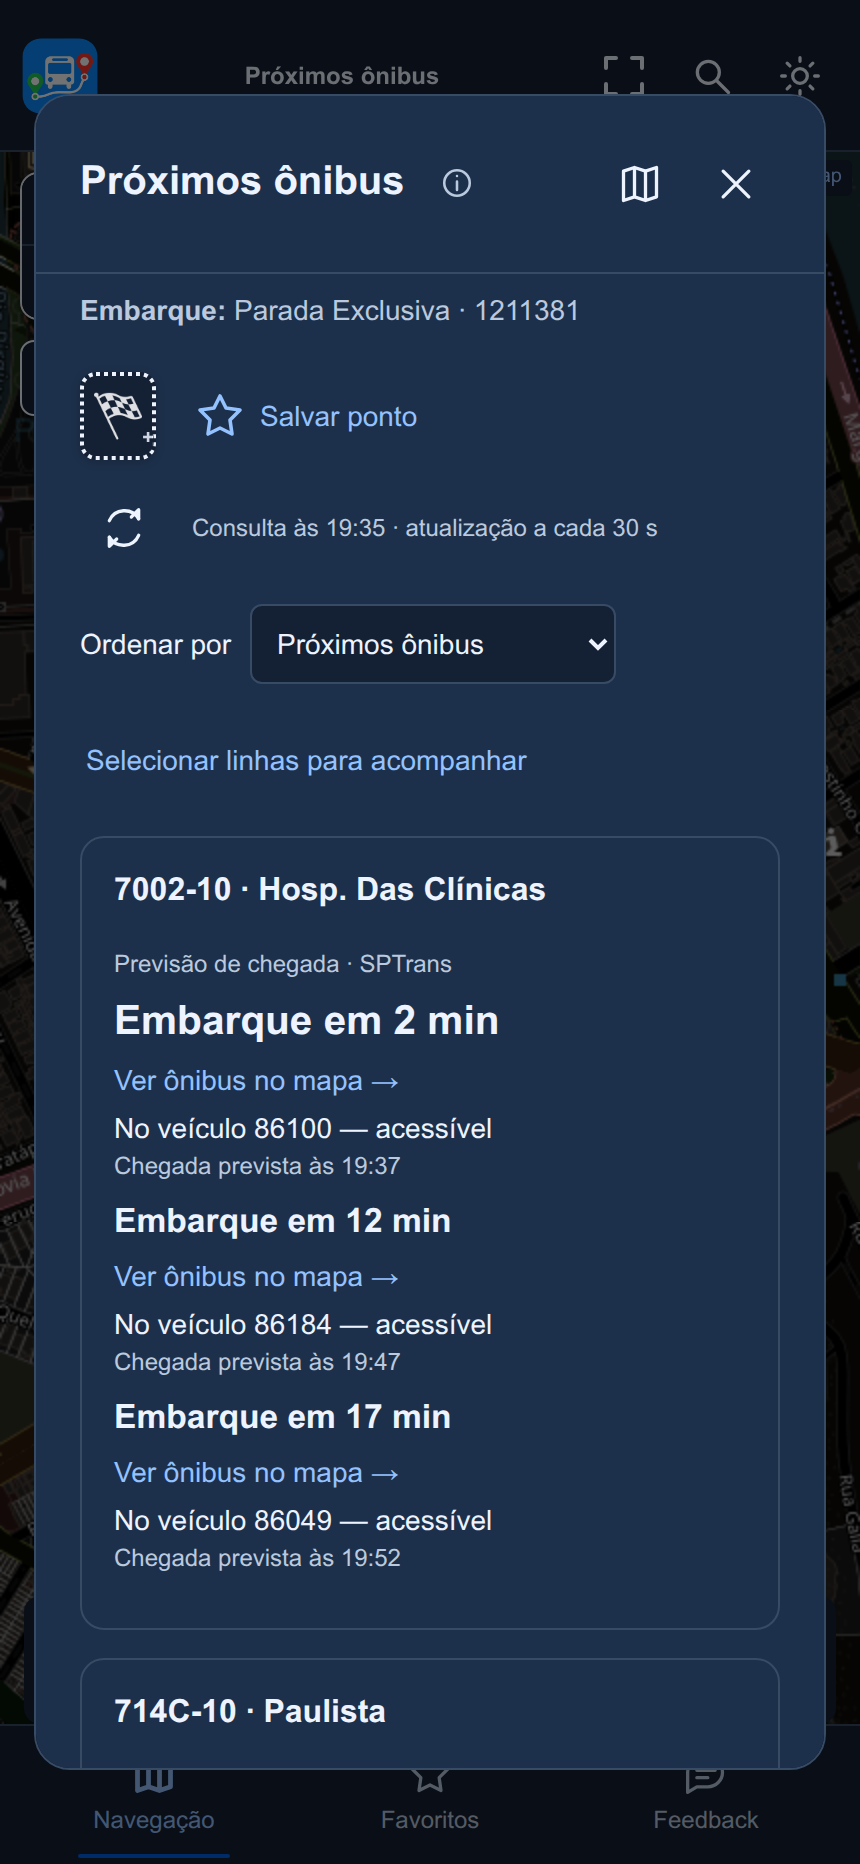
\includegraphics[width=\linewidth]{capturas/2026-10-22/pap-01-embarque.png}
\end{minipage}\hfill
\begin{minipage}[c]{0.60\textwidth}\centering
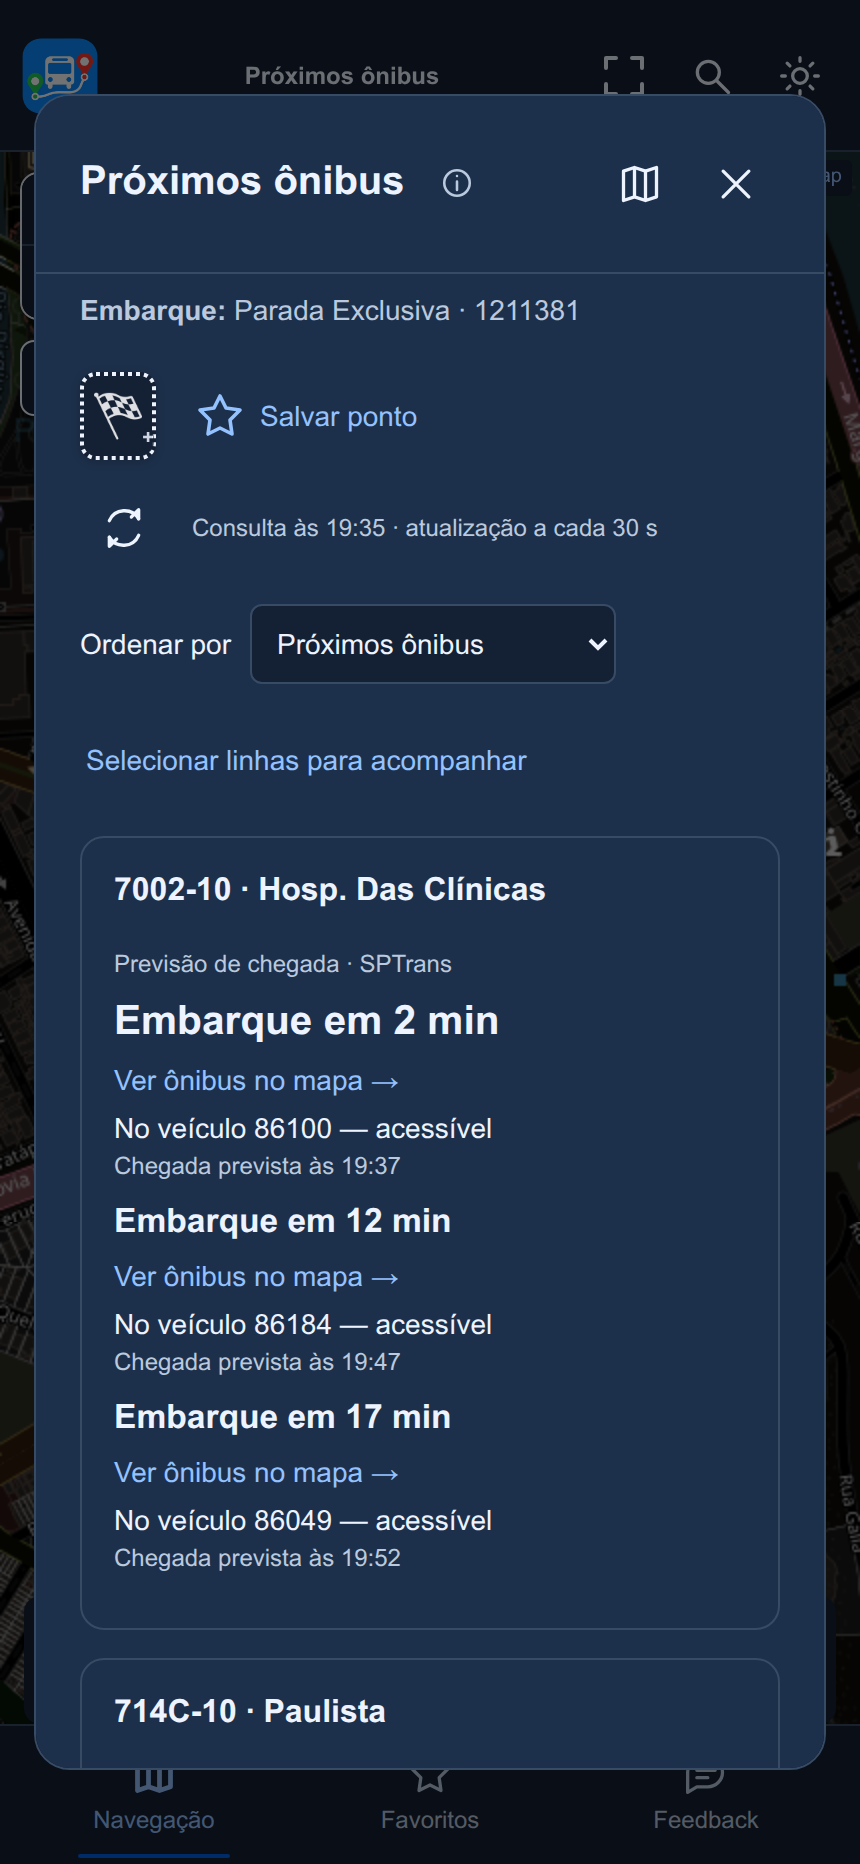
\includegraphics[width=\linewidth,trim=75bp 224bp 70bp 820bp,clip]{capturas/2026-10-22/pap-01-embarque.png}
\small Detalhe ampliado da mesma captura.
\end{minipage}
\caption{Consulta dos próximos ônibus: tela completa e detalhe das previsões.}\label{fig:print-01-embarque}
\fonte{Captura da aplicação em emulação móvel, 22 out. 2026.}
\end{figure}
A consulta foi aberta pelo endereço local da Parada Exclusiva (1211381), no Butantã. O painel distingue previsões operacionais e informações programadas. Os horários são os retornados na captura e não constituem promessa de chegada.
\clearpage

\begin{figure}[H]\centering
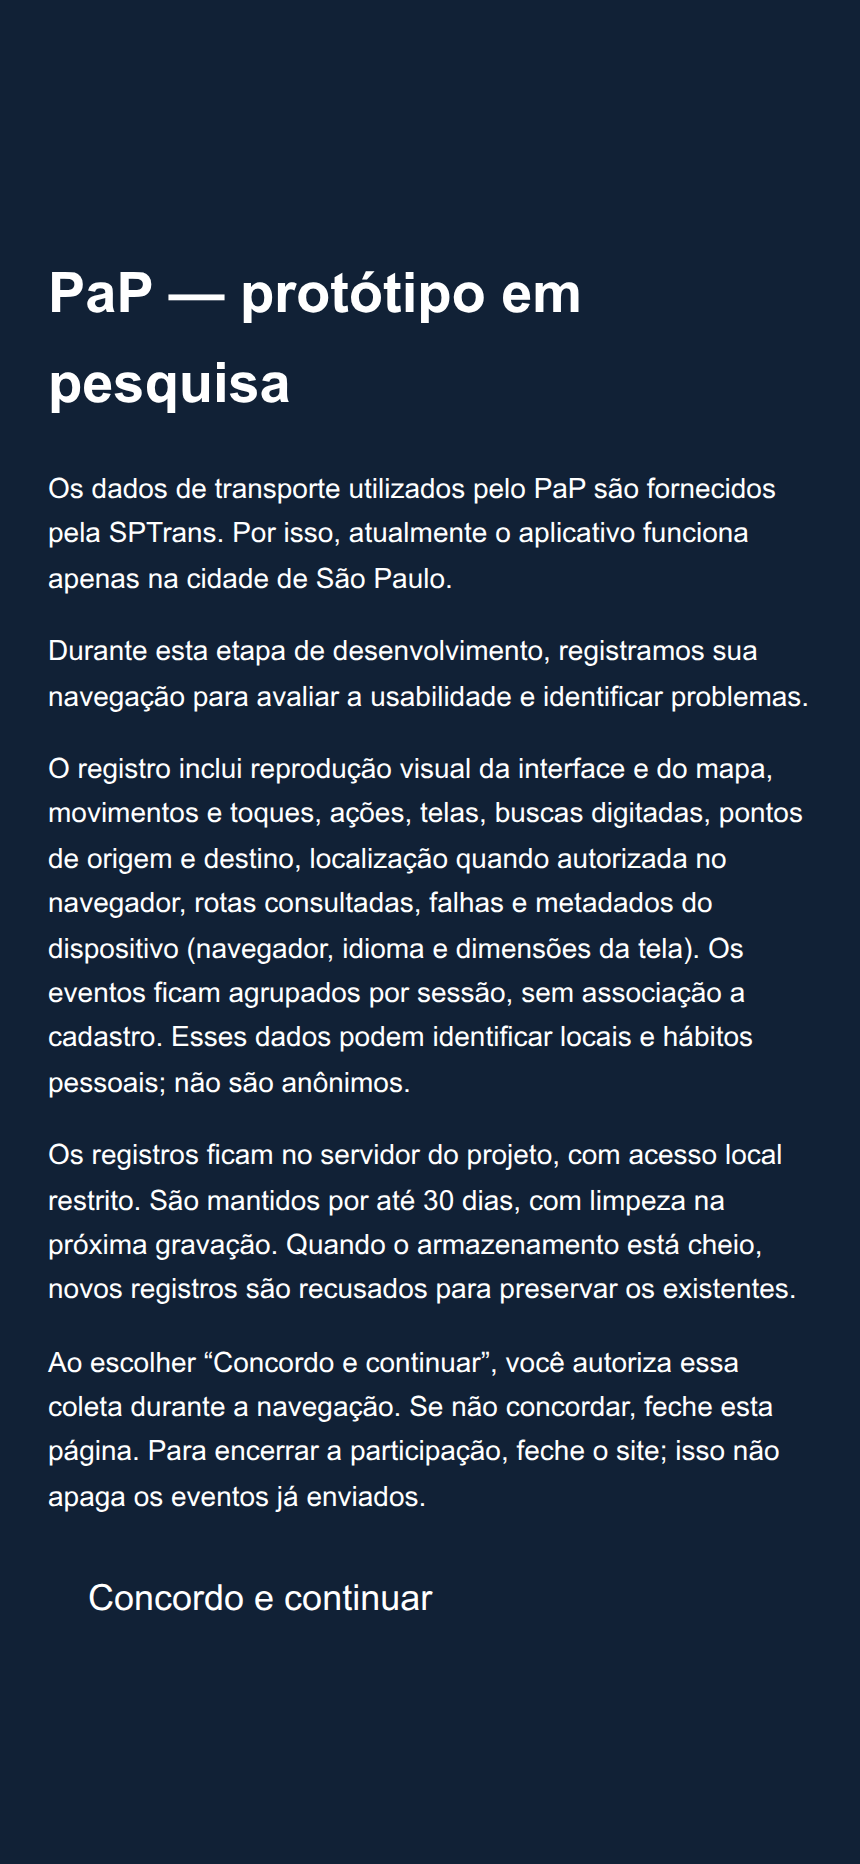
\includegraphics[width=0.80\textwidth,height=0.69\textheight,keepaspectratio,trim=30bp 200bp 30bp 250bp,clip]{capturas/2026-10-22/pap-00-aceite.png}
\caption{Aviso inicial sobre cobertura geográfica e coleta de dados de navegação (recorte das margens vazias).}\label{fig:print-02-informacoes}
\fonte{Captura da aplicação em emulação móvel, 22 out. 2026.}
\end{figure}
O aceite informa que os dados de transporte são fornecidos pela SPTrans e que o PaP funciona atualmente apenas na cidade de São Paulo. A tela também explica os registros de pesquisa e solicita a concordância antes de iniciar a navegação. Esta captura substitui a antiga ilustração conceitual de instalação de uma placa; não houve registro de instalação física.
\clearpage

\begin{figure}[H]\centering
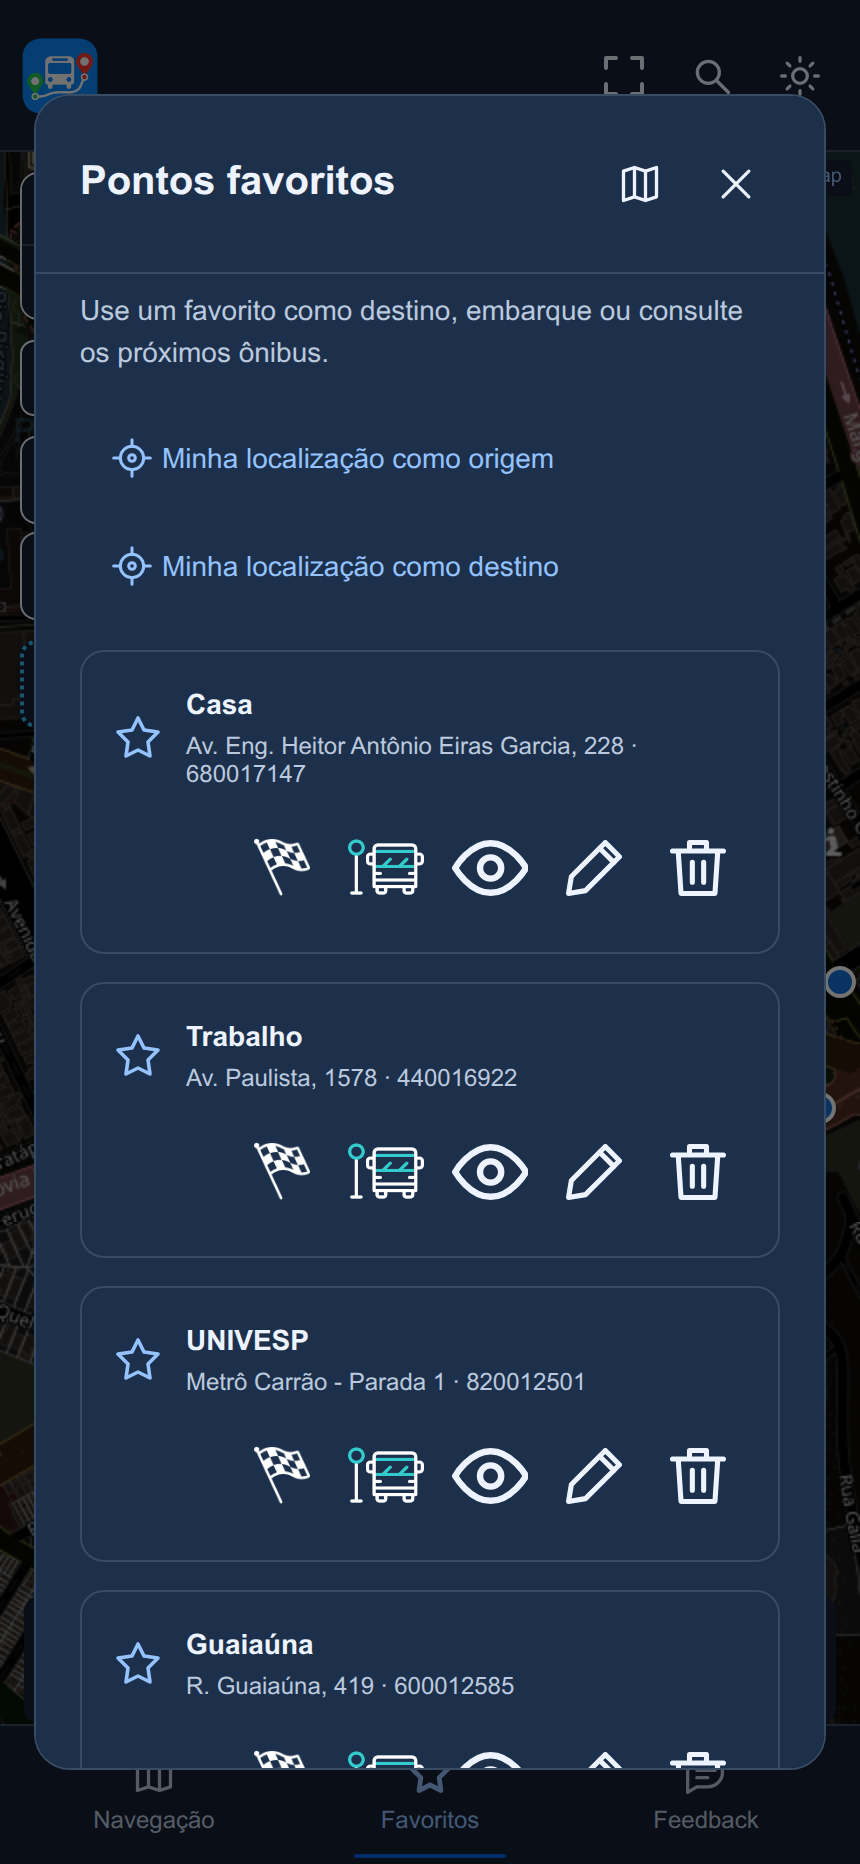
\includegraphics[width=0.80\textwidth,height=0.68\textheight,keepaspectratio]{capturas/2026-10-22/pap-03-destino.png}
\caption{Seleção de destino por pontos favoritos.}\label{fig:print-03-destino}
\fonte{Captura da aplicação em emulação móvel, 22 out. 2026.}
\end{figure}
Os favoritos foram preparados para a documentação com pontos reais e nomes ilustrativos: Casa, Trabalho, UNIVESP e Guaiaúna. Os atalhos permitem escolher destino, embarque ou consulta de próximos ônibus.
\clearpage

\begin{figure}[H]\centering
\begin{minipage}[c]{0.36\textwidth}\centering
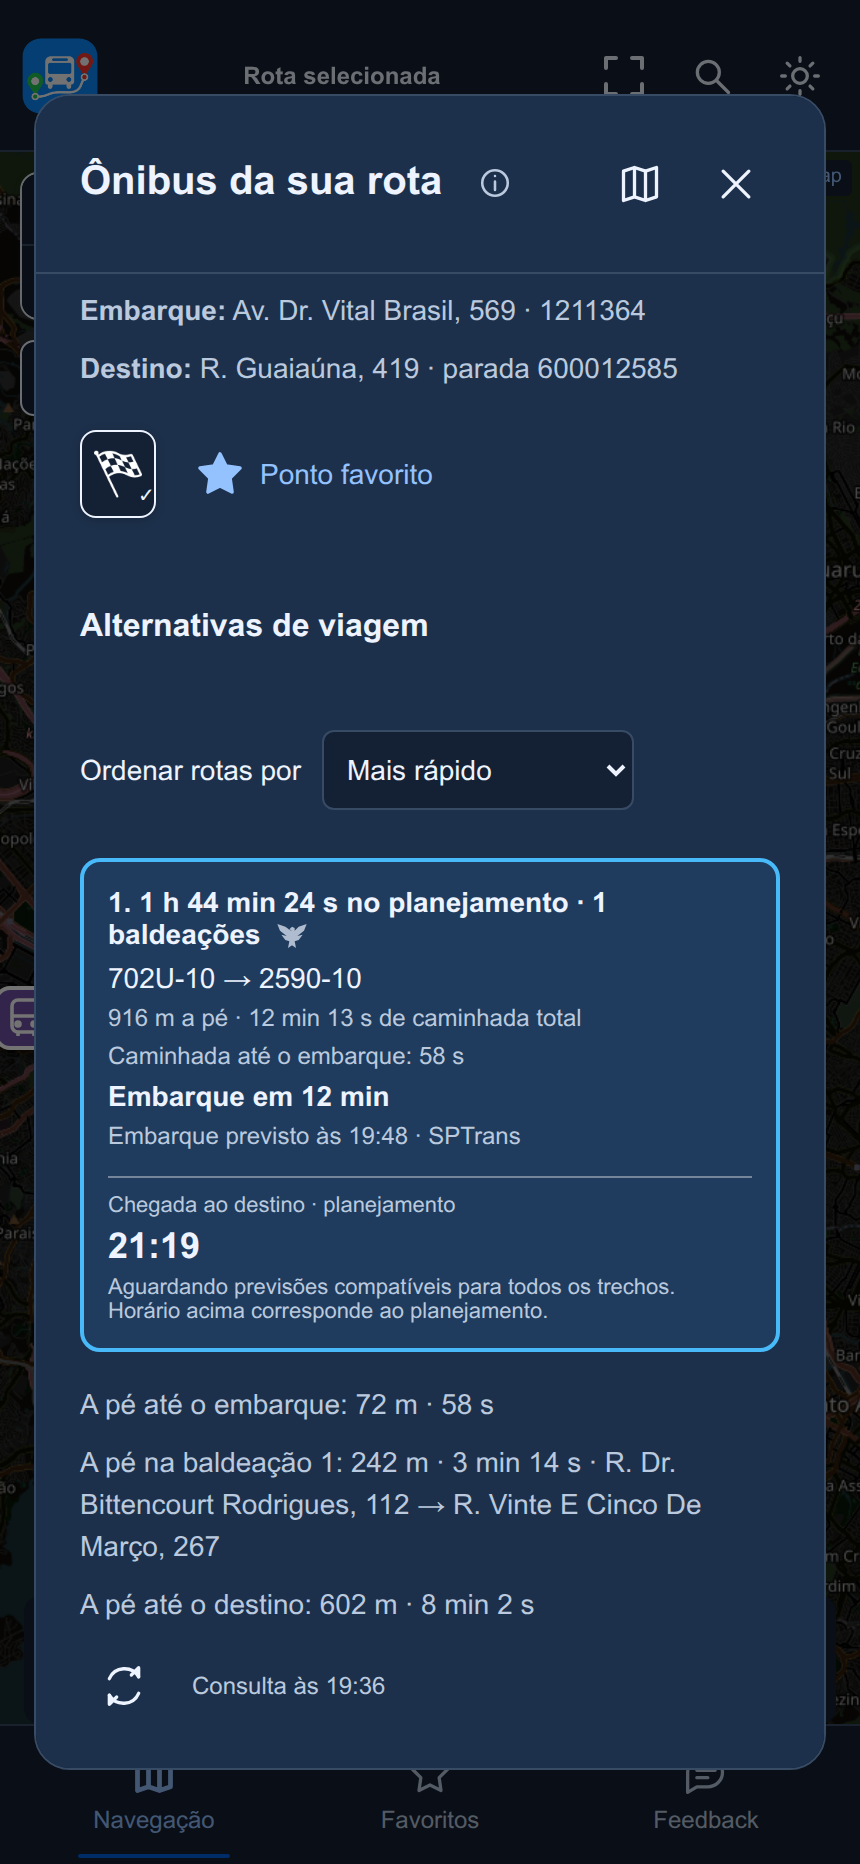
\includegraphics[width=\linewidth]{capturas/2026-10-22/pap-04-alternativas.png}
\end{minipage}\hfill
\begin{minipage}[c]{0.60\textwidth}\centering
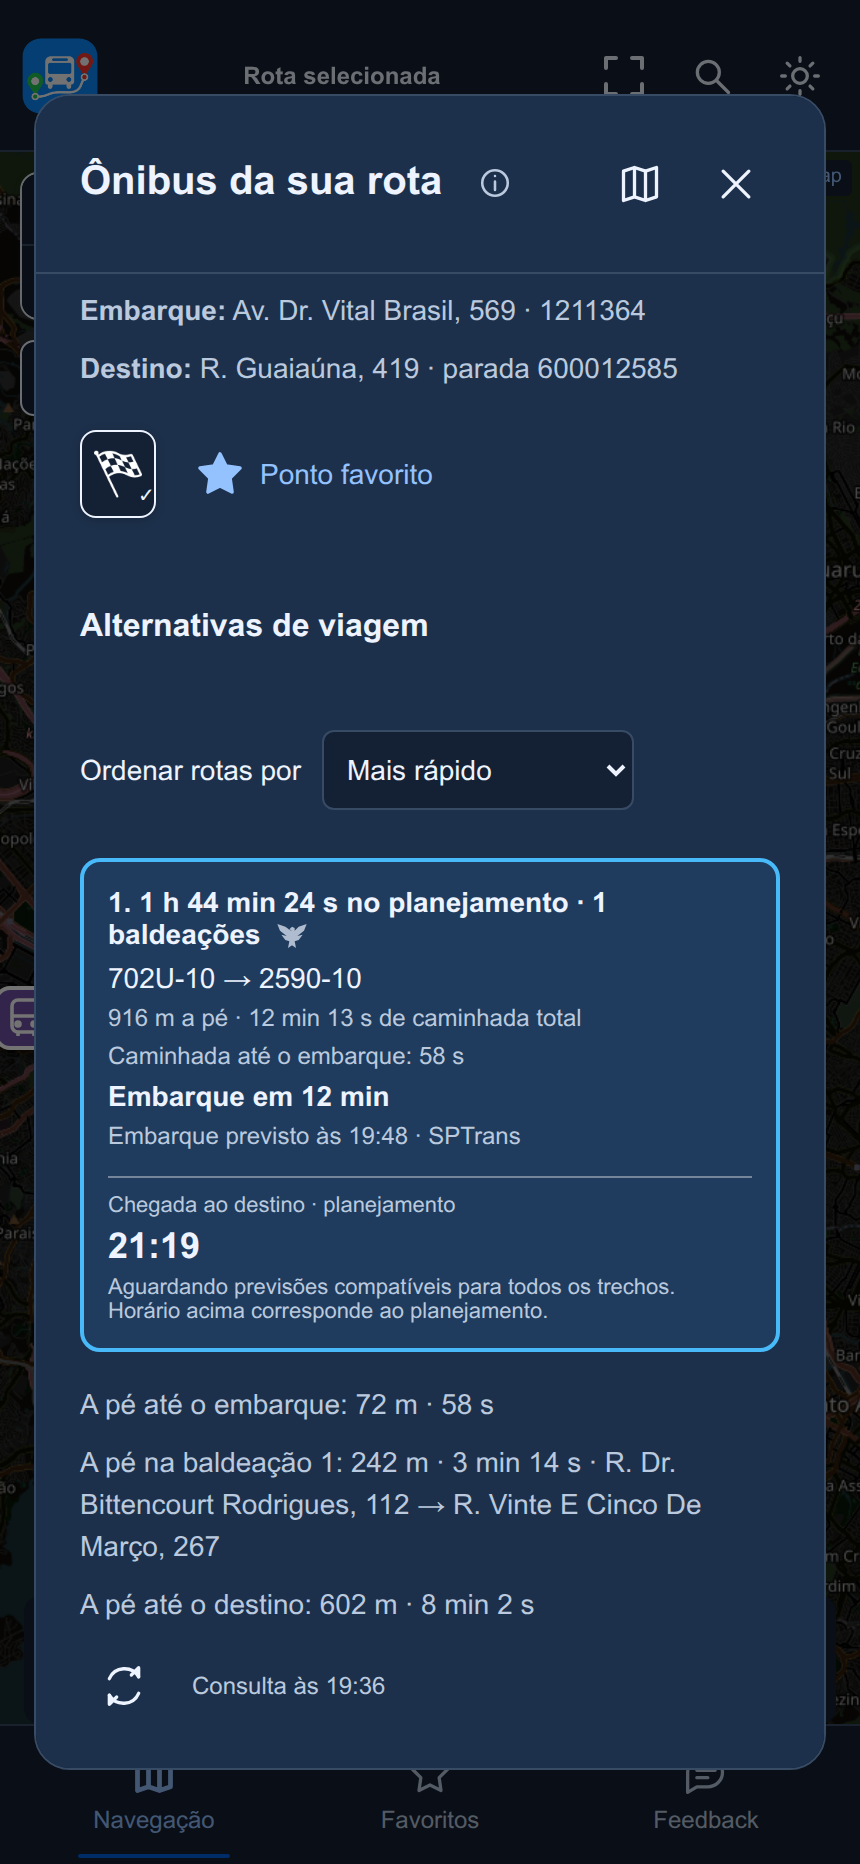
\includegraphics[width=\linewidth,trim=75bp 504bp 70bp 850bp,clip]{capturas/2026-10-22/pap-04-alternativas.png}
\small Detalhe ampliado da mesma captura.
\end{minipage}
\caption{Alternativas de viagem: tela completa e detalhe da alternativa selecionada.}\label{fig:print-04-alternativas}
\fonte{Captura da aplicação em emulação móvel, 22 out. 2026.}
\end{figure}
As capturas integram a mesma sequência registrada no roteiro de captura: acesso à Parada Exclusiva (1211381), retorno ao mapa e seleção de Guaiaúna como destino favorito. O painel de alternativas mostra o embarque do primeiro trecho da rota selecionada, na Av. Dr. Vital Brasil, 569 (1211364), e o destino na Rua Guaiaúna, 419 (600012585). A caminhada de acesso exibida é de 72 m, estimada em 58 s; portanto, o embarque da alternativa difere do ponto usado para iniciar a consulta. O painel apresenta as alternativas calculadas no instante da consulta, com caminhada, baldeações e informações de embarque. Os resultados variam com o horário e com os dados disponíveis.
\clearpage

\begin{figure}[H]\centering
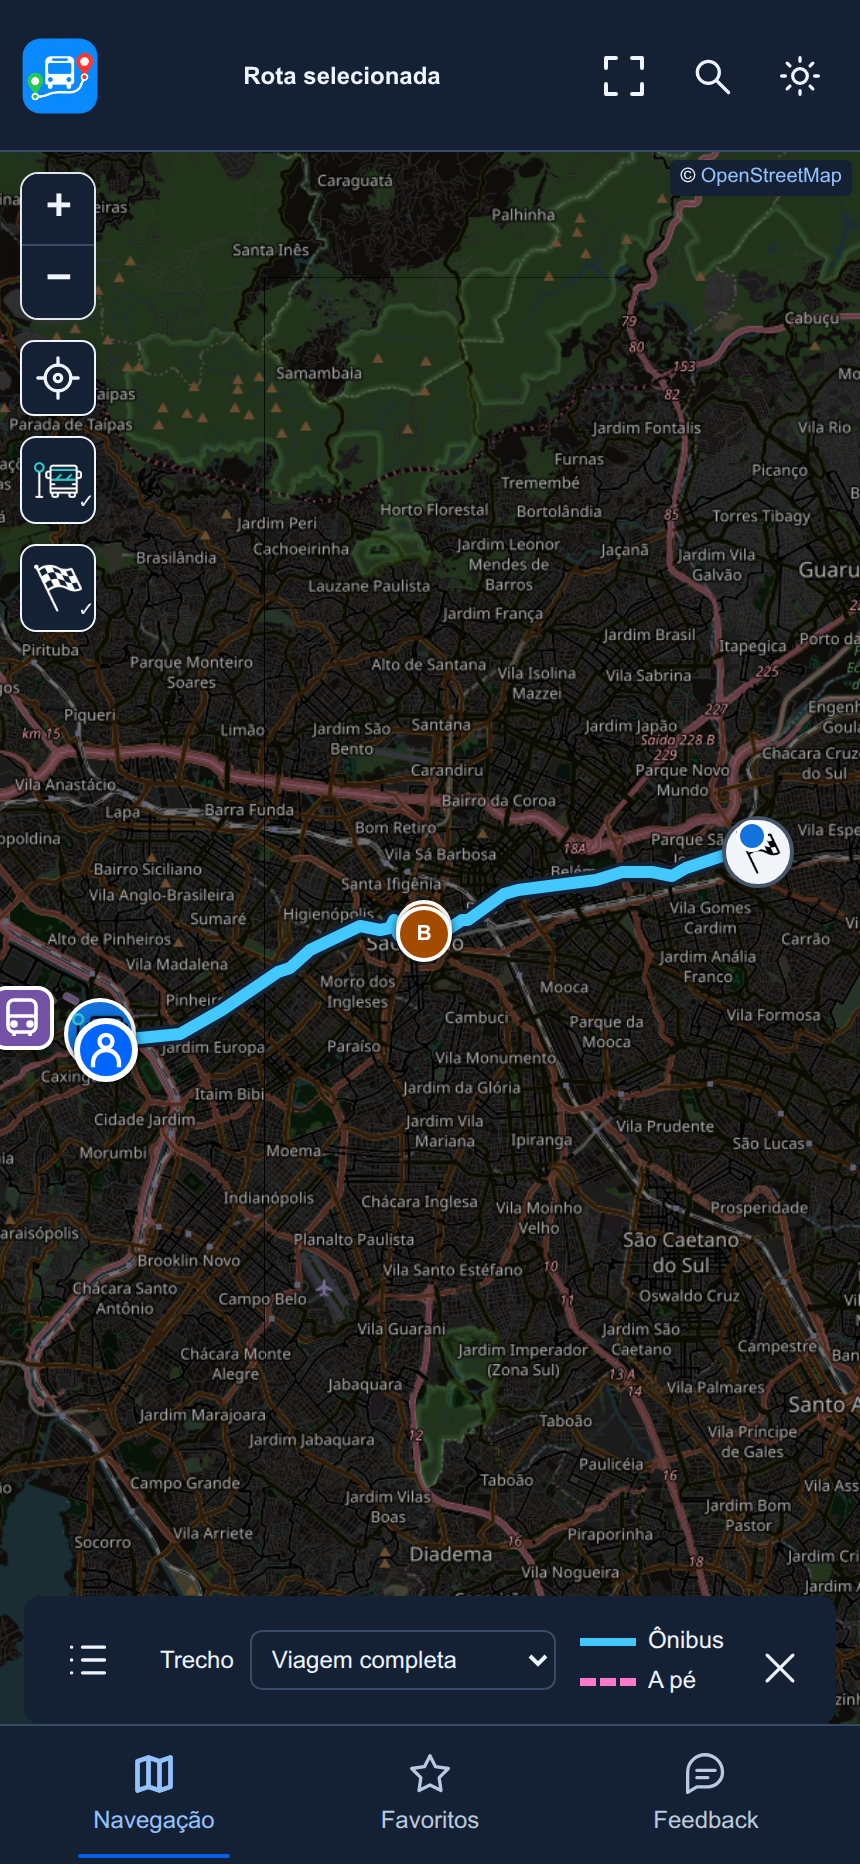
\includegraphics[width=0.80\textwidth,height=0.68\textheight,keepaspectratio]{capturas/2026-10-22/pap-05-viagem-completa.png}
\caption{Viagem completa, com embarque, baldeação e destino.}\label{fig:print-05-viagem-completa}
\fonte{Captura da aplicação em emulação móvel, 22 out. 2026.}
\end{figure}
A rota selecionada é representada no mapa. A legenda distingue trechos de ônibus e caminhada; o controle inferior permite retornar à lista ou selecionar um trecho quando houver baldeação.
\clearpage

\begin{figure}[H]\centering
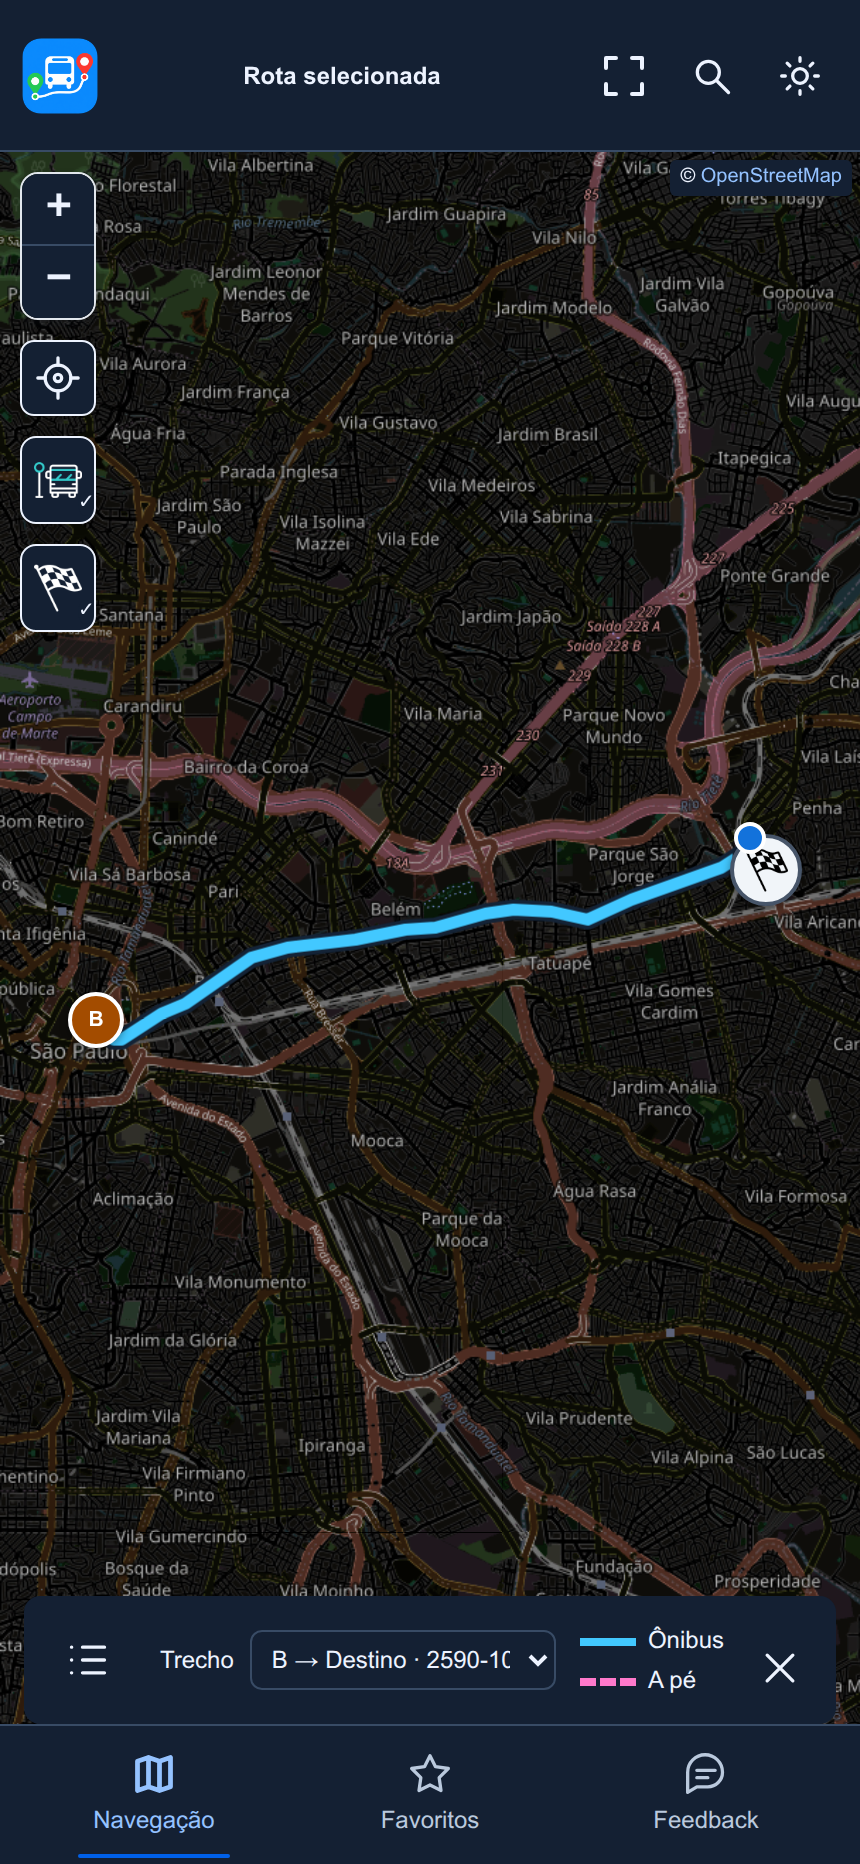
\includegraphics[width=0.80\textwidth,height=0.68\textheight,keepaspectratio]{capturas/2026-10-22/pap-06-ultimo-trecho.png}
\caption{Visualização do último trecho da viagem selecionada.}\label{fig:print-06-ultimo-trecho}
\fonte{Captura da aplicação em emulação móvel, 22 out. 2026.}
\end{figure}
O seletor de trechos permite examinar a parte final do percurso sem perder a referência da viagem escolhida.
\clearpage

\begin{figure}[H]\centering
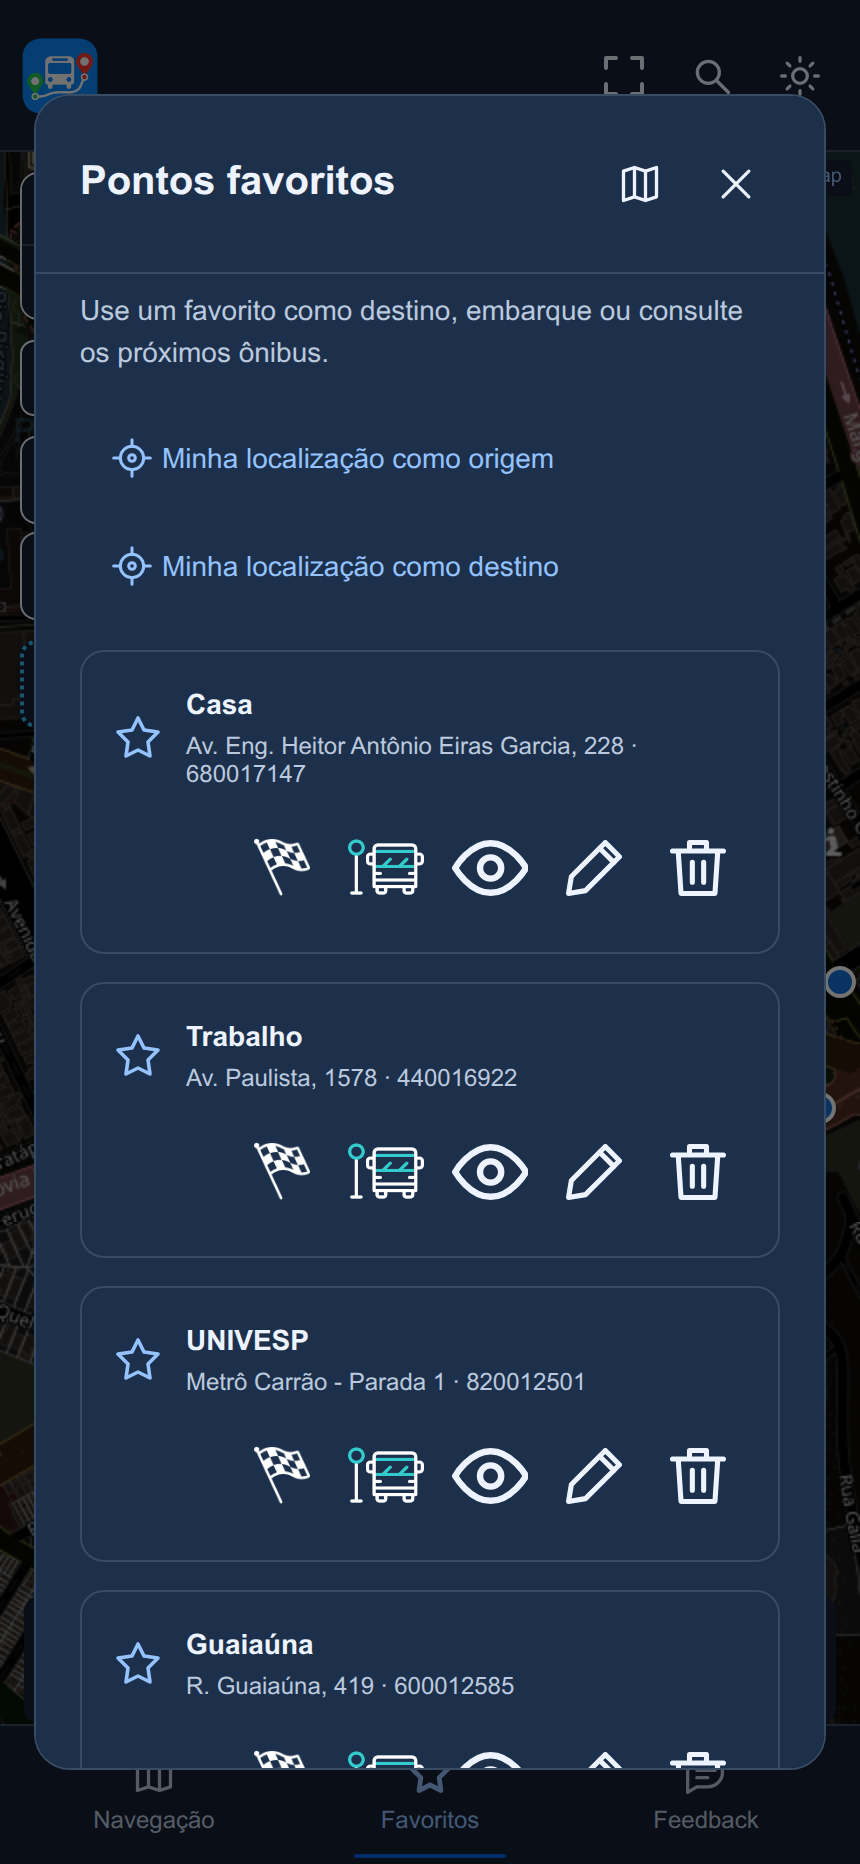
\includegraphics[width=0.80\textwidth,height=0.68\textheight,keepaspectratio]{capturas/2026-10-22/pap-07-favoritos.png}
\caption{Favoritos nomeados e ações disponíveis para cada ponto.}\label{fig:print-07-favoritos}
\fonte{Captura da aplicação em emulação móvel, 22 out. 2026.}
\end{figure}
Os ícones oferecem ações de destino, embarque, consulta, renomeação e remoção. Os nomes salvos para esta captura são exemplos de organização pessoal.
\clearpage

\begin{figure}[H]\centering
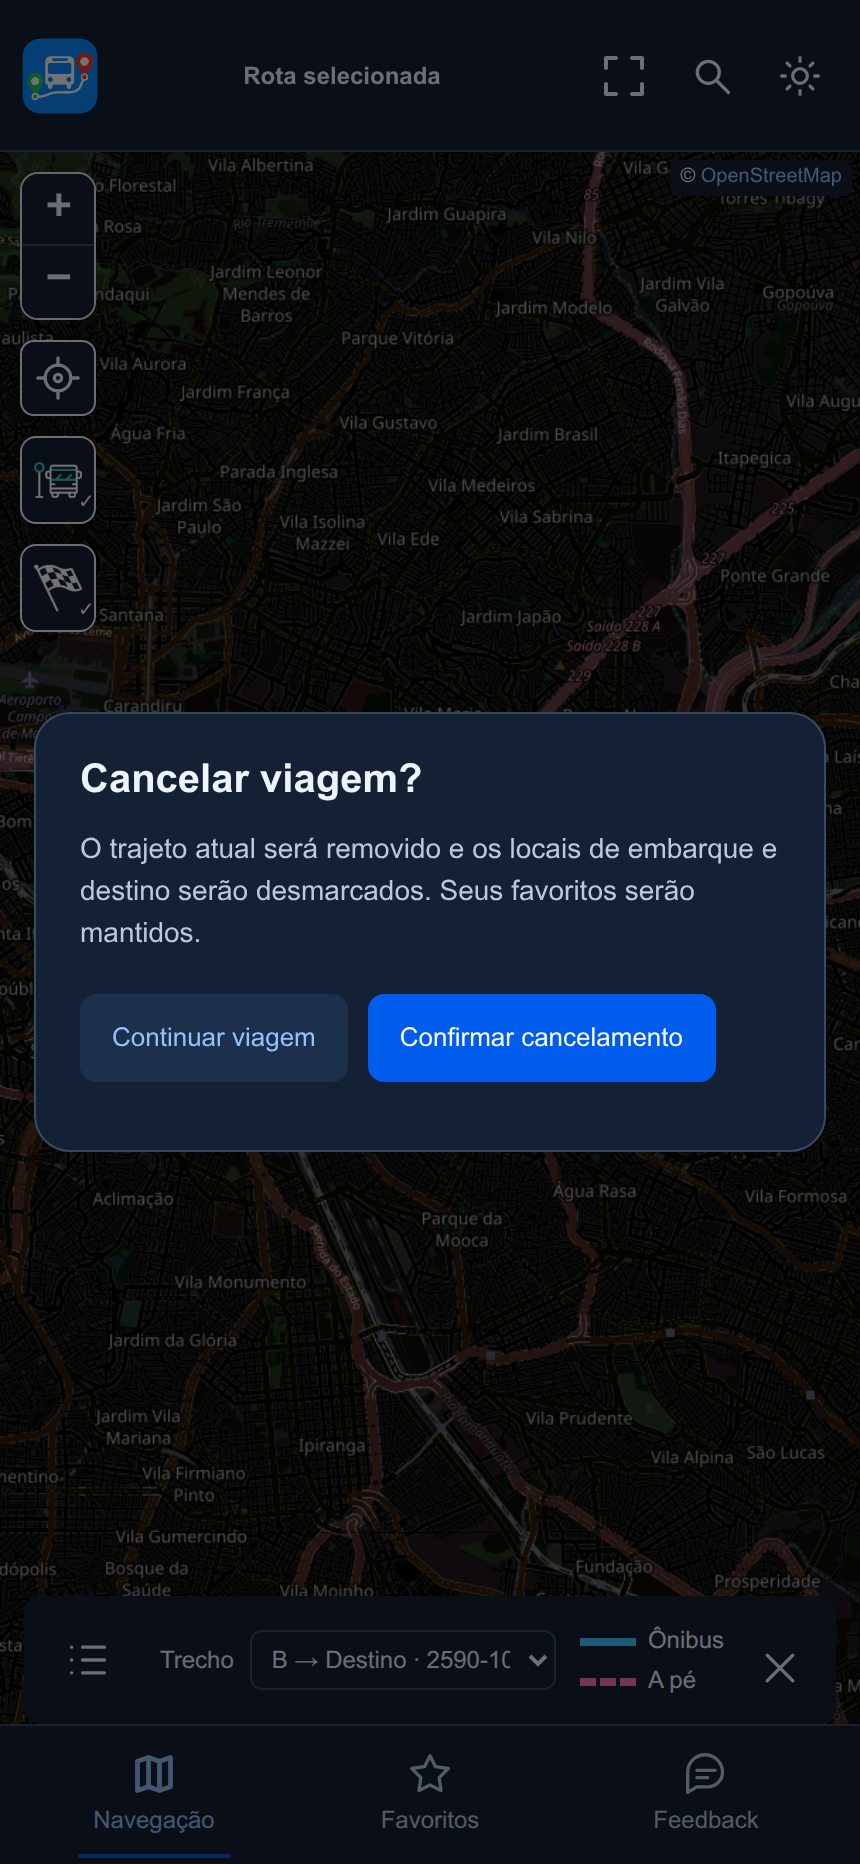
\includegraphics[width=0.80\textwidth,height=0.68\textheight,keepaspectratio]{capturas/2026-10-22/pap-08-confirmacao.png}
\caption{Confirmação antes de cancelar a viagem.}\label{fig:print-08-confirmacao}
\fonte{Captura da aplicação em emulação móvel, 22 out. 2026.}
\end{figure}
O diálogo explica que o trajeto e os locais de embarque e destino serão desmarcados, preservando os favoritos. O passageiro pode continuar a viagem ou confirmar o cancelamento.
\clearpage

\begin{figure}[H]\centering
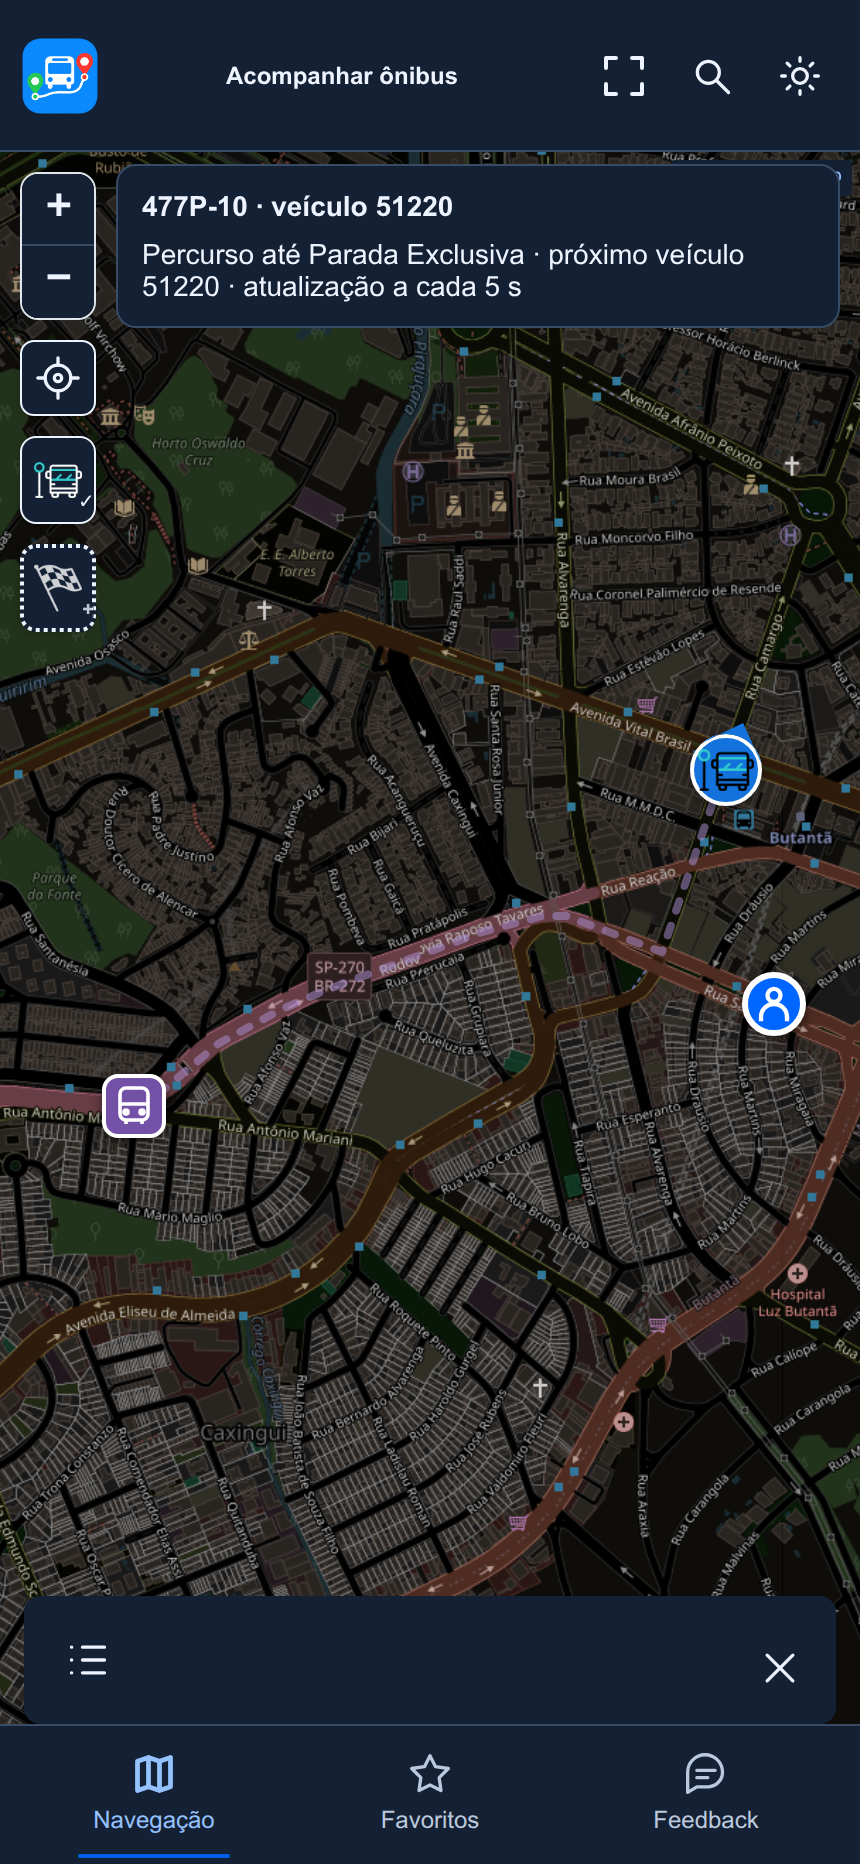
\includegraphics[width=0.80\textwidth,height=0.68\textheight,keepaspectratio]{capturas/2026-10-22/pap-13-onibus-tempo-real.png}
\caption{Acompanhamento de veículo consultado na API Olho Vivo.}\label{fig:print-onibus-tempo-real}
\fonte{Captura da aplicação em emulação móvel, 22 out. 2026.}
\end{figure}
A tela foi aberta pela ação de visualizar um veículo na consulta dos próximos ônibus. O marcador utiliza a posição disponível no serviço externo no momento da captura. Uma imagem estática não comprova atualização periódica nem precisão operacional.
\clearpage
\begin{figure}[H]\centering
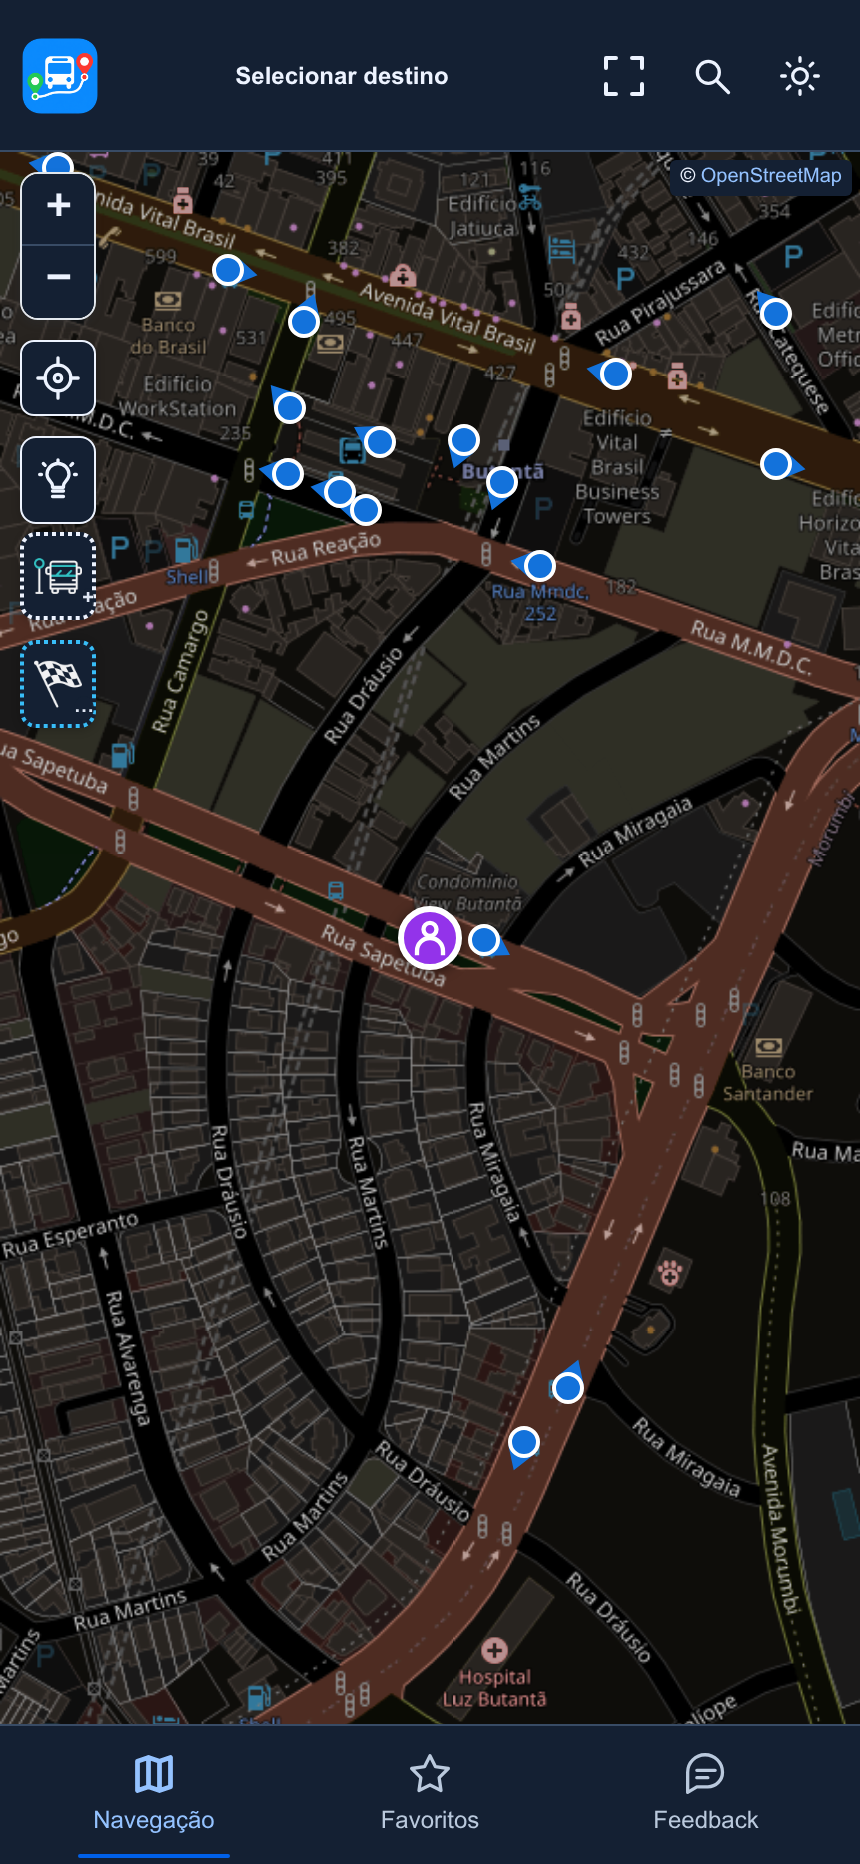
\includegraphics[width=0.43\textwidth,height=0.60\textheight,keepaspectratio]{capturas/2026-10-22/pap-09-localizacao.png}\hfill
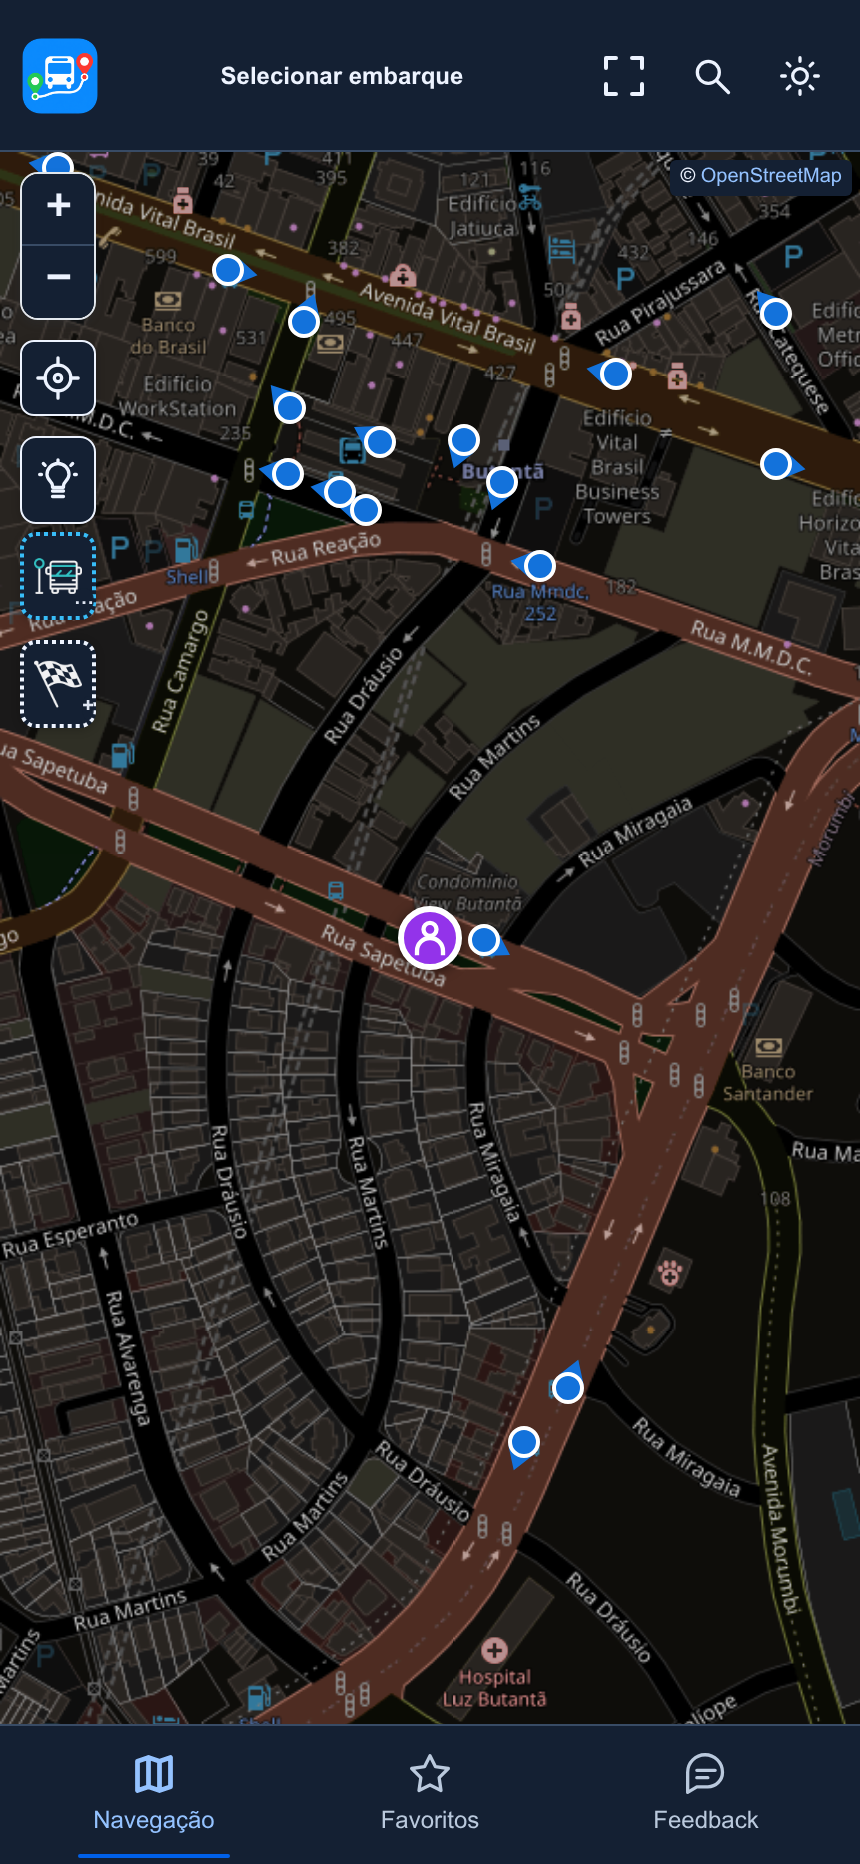
\includegraphics[width=0.43\textwidth,height=0.60\textheight,keepaspectratio]{capturas/2026-10-22/pap-10-alterar-embarque.png}
\caption{Localização simulada como origem (à esquerda) e seleção manual do embarque (à direita).}\label{fig:print-localizacao}
\fonte{Capturas da aplicação em emulação móvel, 22 out. 2026.}
\end{figure}
O marcador roxo indica a localização simulada. O controle lateral permite escolher uma parada de embarque no mapa. O cabeçalho utiliza a expressão Selecionar embarque; a navegação inferior inclui o acesso ao feedback.
\clearpage

\begin{figure}[H]\centering
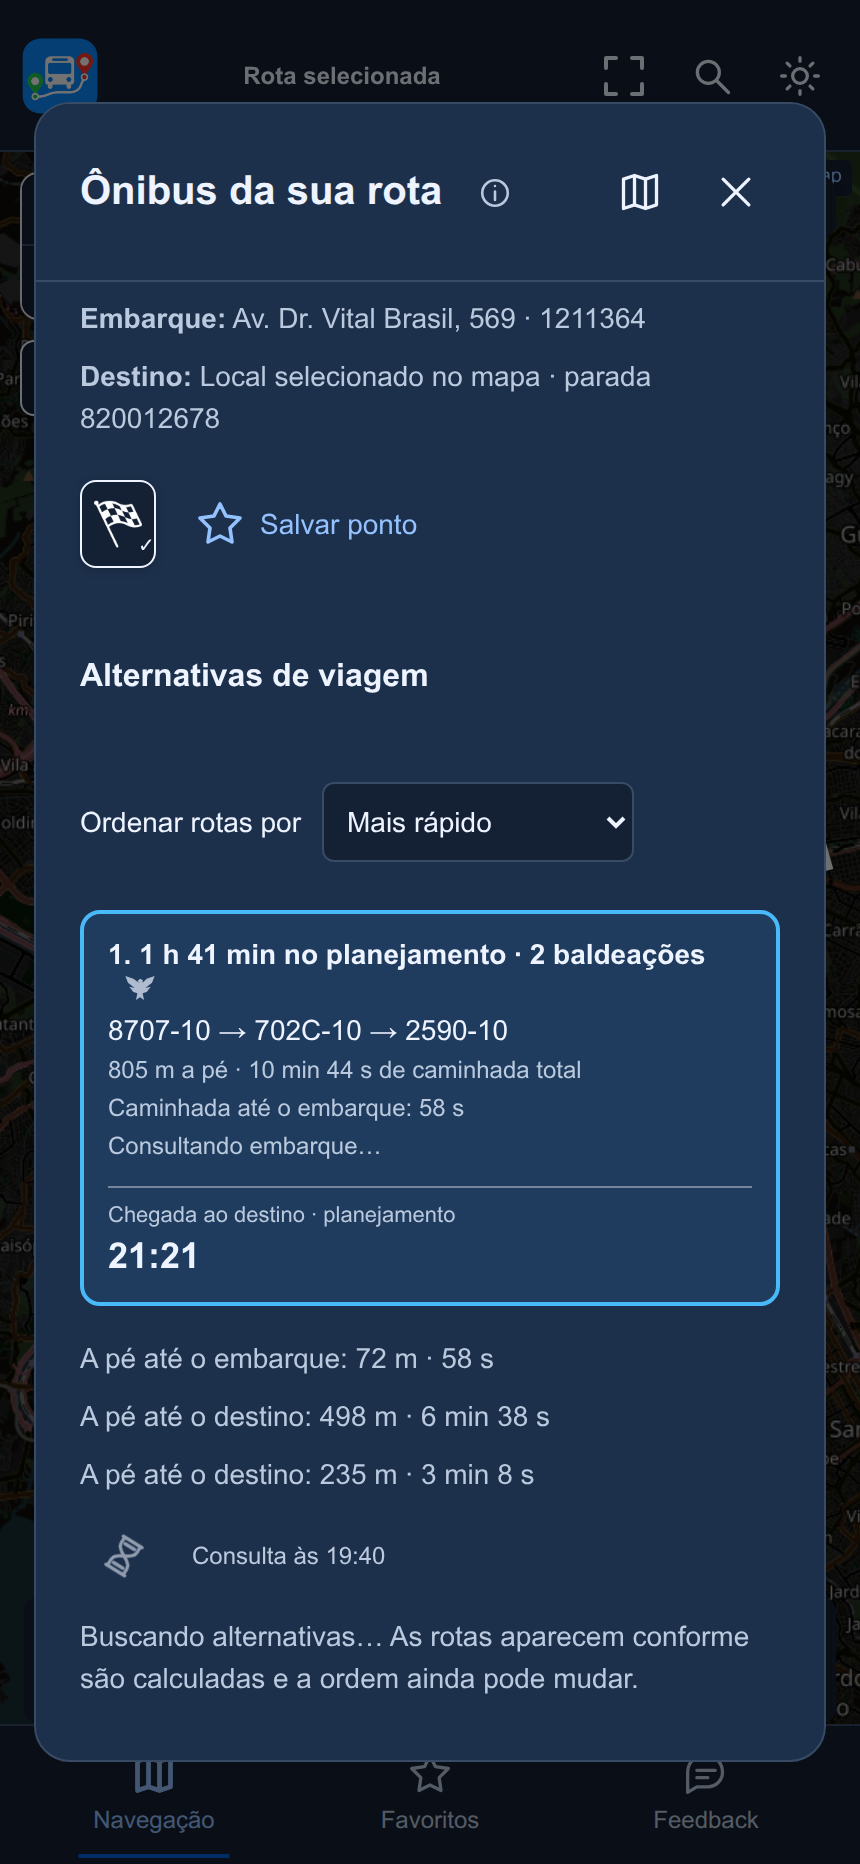
\includegraphics[width=0.80\textwidth,height=0.68\textheight,keepaspectratio]{capturas/2026-10-22/pap-12-destino-livre.png}
\caption{Destino definido por toque prolongado no mapa.}\label{fig:print-destino-livre}
\fonte{Captura da aplicação em emulação móvel, 22 out. 2026.}
\end{figure}
A busca por coordenadas centralizou a região desejada e o toque prolongado definiu um local de destino. O painel apresenta alternativas progressivamente e, no instante capturado, ainda consulta informações de embarque. A imagem não representa o encerramento de todas as consultas.
\clearpage

\begin{figure}[H]\centering
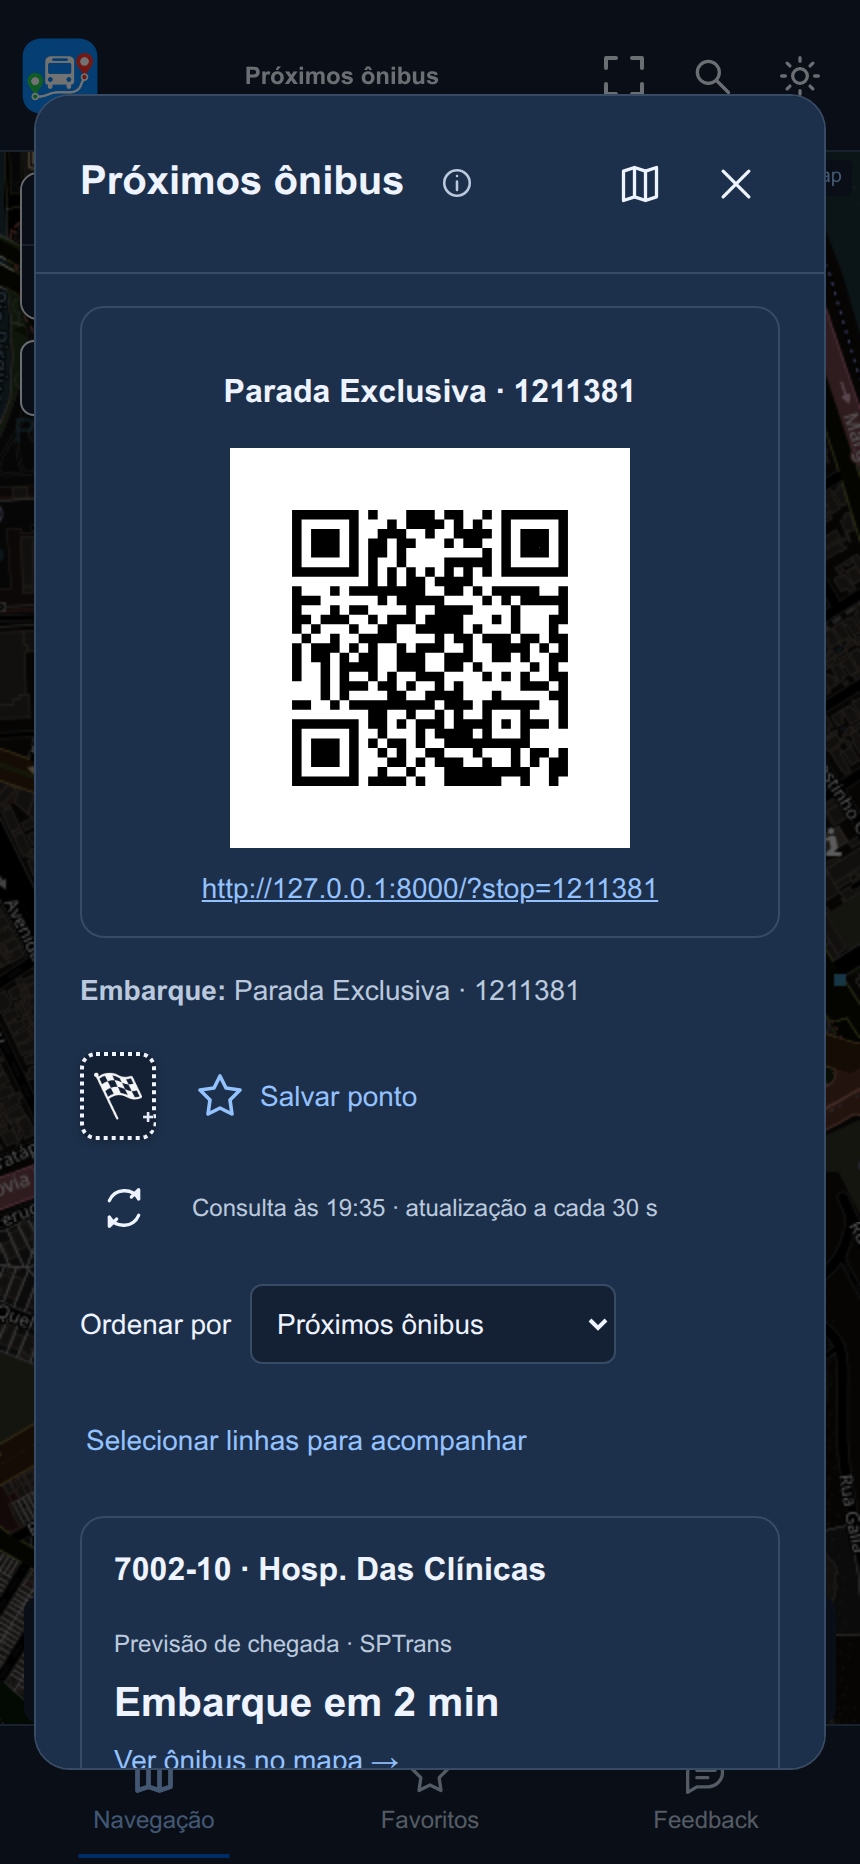
\includegraphics[width=0.80\textwidth,height=0.68\textheight,keepaspectratio]{capturas/2026-10-22/pap-14-qr-atual.png}
\caption{Informações da parada e QR Code de acesso à consulta.}\label{fig:print-qr-atual}
\fonte{Captura da aplicação em emulação móvel, 22 out. 2026.}
\end{figure}
A tela utiliza o identificador 1211381 e o endereço local de desenvolvimento. A captura documenta a geração do QR Code; não demonstra leitura física pela câmera. Para uso externo, é necessário um endereço HTTPS acessível aos passageiros.
\clearpage
